\textbf{TO BE COMPLETED}\\
\vspace{0.5cm}
%\textbf{TO BE COMPLETED}\\
\vspace{0.5cm}
%\textbf{TO BE COMPLETED}\\
\vspace{0.5cm}
%\textbf{TO BE COMPLETED}\\
\vspace{0.5cm}
%\input{HowToAddRules}
There are three ways to add a new rule to the Modelbase: 1) add a rule to a list of common monetary policy rules, 2) include the model-specific rule calibrated or estimated by the original model authors and 3) specify a rule using the Modelbase user-specified rule option. Below we discuss each case in detail. Keep in mind that policy rules in the Modelbase have to be reformulated in terms of common Modelbase variables such as the annualized quarterly interest rate, the annualized quarter-to-quarter rate of inflation, the quarterly output and the quarterly output gap. This is explained in detail in \cite{WCMSW2012} and in the separate document, called 'MMB\_MPrule\_description.pdf'. Also, one can see how it practically works by looking at common monetary policy rules already implemented in the \emph{MMB\_OPTIONS/MMB\_settings.m} file.
\newline


\noindent {\it 1) Add a common monetary policy rule}\\
\textbf{TO BE COMPLETED}
\begin{itemize}
  \item The first task is to choose a suitable name for the new policy rule and to include it into an array for a list of rule names, \emph{rulenames}. One also has to add its acronyms in character arrays, \emph{rulenamesshort} and \emph{rulenamesshort1} \footnote{ As \emph{rulenamesshort1} are used for displaying simulation outcomes in Matlab console, any blank is not allowed in the rule name.}. Please make sure that the new rule name is of the same size of character array as the already existing one. Next, one assigns color to the rule with the array \textit{myrulecolor}.
	\item Then, one adds the specification of the new-rule coefficients right after the last common rule's specification.
  \item The remaining work is to add the new rule to the frontend of the MMB 3.0 \\\textbf{TO BE COMPLETED}.
\end{itemize}


\noindent {\it 2) Add the model-specific monetary policy rule}

\begin{itemize}
  \item When adding a new model, it is possible to include its policy rule as long as the rule can be rewritten in terms of Modelbase common variables. If this is the case, the user should add the model identification number to the variable vector \emph{model\_with\_rule} in the  file \emph{MMB\_settings.m} such that a model-specific rule is activated when its corresponding model is chosen in \textbf{Option 2}. Otherwise, the user should add the model number to the variable vector \emph{model\_without\_rule}. For example, if the policy rule is set for the interest rate to react to exchange rate or credit growth, the user cannot include the original rule in the Modelbase.
  \item Finally, the user has to insert the specification of the model-specific rule into the part of \emph{switch} statement in the file \emph{MMB\_OPTIONS/MSR\_COEFFFS.m} using the model's identification number as the case expression.
\end{itemize}

\noindent {\it 3) User-specified monetary rule}

\begin{itemize}
  \item When \textit{User-specified rule} is chosen, a menu with a general form of a monetary policy rule appears in terms of common variables. Then, one can specify desired coefficient values of each variable in columns and to the corresponding lag/lead in rows.
      For example, to implement the Taylor (1993) rule using the option for user-specified monetary policy rule, one should set the coefficients as following: $ \rho_{\pi,0} = \rho_{\pi,-1} = \rho_{\pi,-2} = \rho_{\pi,-3} = 0.375, \rho_{q,0} = 0.5 $ and the rest of coefficients to zero. Figure \ref{img:userruletaylor} illustrates how to use the option for a user-specified rule with the example of Taylor (1993) rule. \\

        \begin{figure}[H]
        \centering
        \caption{\textsc{Taylor (1993) rule using the option of user-specified rule }}
        \vspace{0.2cm}
        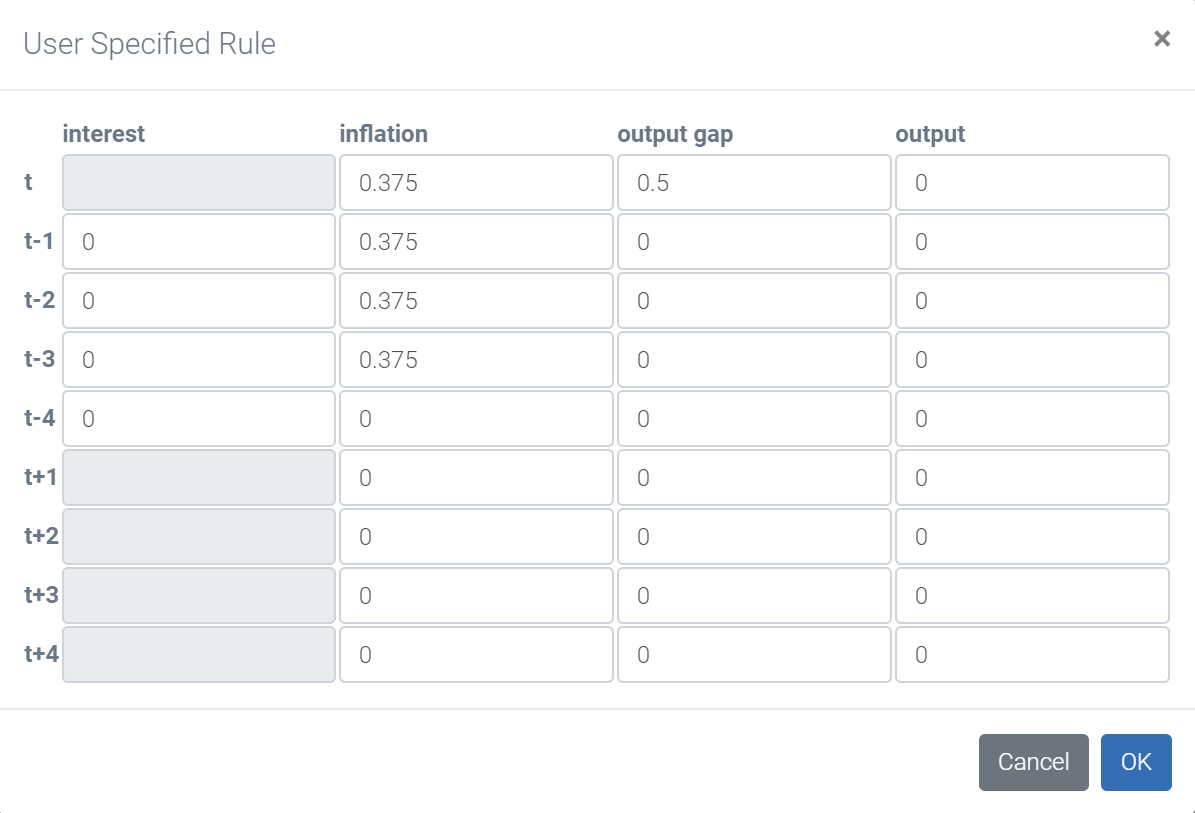
\includegraphics[width=13cm,keepaspectratio]{userrule.png}
        \label{img:userruletaylor}
        \end{figure}

  \item Note that with certain rule parametrization, models cannot be solved due to several reasons. For example, the system of equations may violate the Blanchard-Kahn conditions so a model does not yield a unique stationary rational expectations equilibrium. There is no clear guideline for conditions for determinacy, but \cite{LevinWielandWilliams2003} suggest several crucial characteristics of rules that deliver a unique equilibrium: a relatively short inflation forecast horizon, a moderate degree of responsiveness to the inflation forecast, an explicit response to the current output gap, and a substantial degree of policy inertia.
\end{itemize}


There are three ways to add a new rule to the Modelbase: 1) add a rule to a list of common monetary policy rules, 2) include the model-specific rule calibrated or estimated by the original model authors and 3) specify a rule using the Modelbase user-specified rule option. Below we discuss each case in detail. Keep in mind that policy rules in the Modelbase have to be reformulated in terms of common Modelbase variables such as the annualized quarterly interest rate, the annualized quarter-to-quarter rate of inflation, the quarterly output and the quarterly output gap. This is explained in detail in \cite{WCMSW2012} and in the separate document, called 'MMB\_MPrule\_description.pdf'. Also, one can see how it practically works by looking at common monetary policy rules already implemented in the \emph{MMB\_OPTIONS/MMB\_settings.m} file.
\newline


\noindent {\it 1) Add a common monetary policy rule}\\
\textbf{TO BE COMPLETED}
\begin{itemize}
  \item The first task is to choose a suitable name for the new policy rule and to include it into an array for a list of rule names, \emph{rulenames}. One also has to add its acronyms in character arrays, \emph{rulenamesshort} and \emph{rulenamesshort1} \footnote{ As \emph{rulenamesshort1} are used for displaying simulation outcomes in Matlab console, any blank is not allowed in the rule name.}. Please make sure that the new rule name is of the same size of character array as the already existing one. Next, one assigns color to the rule with the array \textit{myrulecolor}.
	\item Then, one adds the specification of the new-rule coefficients right after the last common rule's specification.
  \item The remaining work is to add the new rule to the frontend of the MMB 3.0 \\\textbf{TO BE COMPLETED}.
\end{itemize}


\noindent {\it 2) Add the model-specific monetary policy rule}

\begin{itemize}
  \item When adding a new model, it is possible to include its policy rule as long as the rule can be rewritten in terms of Modelbase common variables. If this is the case, the user should add the model identification number to the variable vector \emph{model\_with\_rule} in the  file \emph{MMB\_settings.m} such that a model-specific rule is activated when its corresponding model is chosen in \textbf{Option 2}. Otherwise, the user should add the model number to the variable vector \emph{model\_without\_rule}. For example, if the policy rule is set for the interest rate to react to exchange rate or credit growth, the user cannot include the original rule in the Modelbase.
  \item Finally, the user has to insert the specification of the model-specific rule into the part of \emph{switch} statement in the file \emph{MMB\_OPTIONS/MSR\_COEFFFS.m} using the model's identification number as the case expression.
\end{itemize}

\noindent {\it 3) User-specified monetary rule}

\begin{itemize}
  \item When \textit{User-specified rule} is chosen, a menu with a general form of a monetary policy rule appears in terms of common variables. Then, one can specify desired coefficient values of each variable in columns and to the corresponding lag/lead in rows.
      For example, to implement the Taylor (1993) rule using the option for user-specified monetary policy rule, one should set the coefficients as following: $ \rho_{\pi,0} = \rho_{\pi,-1} = \rho_{\pi,-2} = \rho_{\pi,-3} = 0.375, \rho_{q,0} = 0.5 $ and the rest of coefficients to zero. Figure \ref{img:userruletaylor} illustrates how to use the option for a user-specified rule with the example of Taylor (1993) rule. \\

        \begin{figure}[H]
        \centering
        \caption{\textsc{Taylor (1993) rule using the option of user-specified rule }}
        \vspace{0.2cm}
        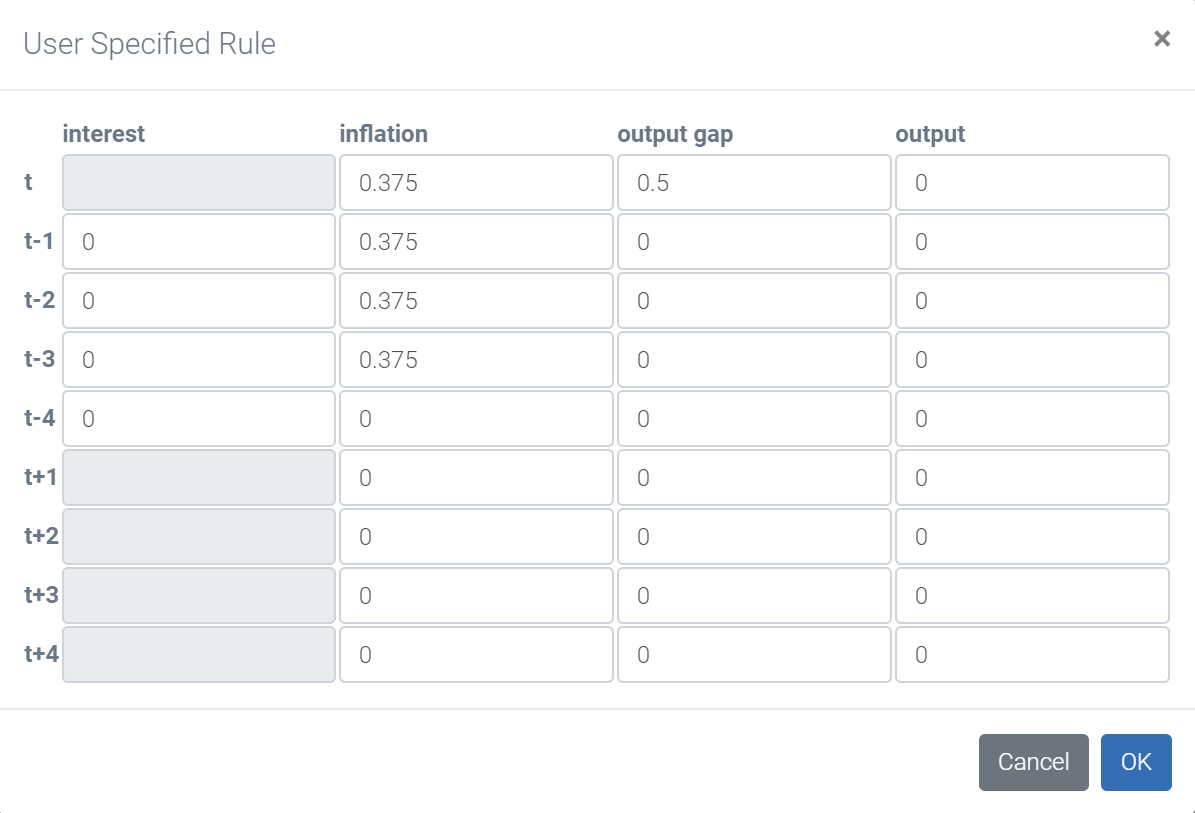
\includegraphics[width=13cm,keepaspectratio]{userrule.png}
        \label{img:userruletaylor}
        \end{figure}

  \item Note that with certain rule parametrization, models cannot be solved due to several reasons. For example, the system of equations may violate the Blanchard-Kahn conditions so a model does not yield a unique stationary rational expectations equilibrium. There is no clear guideline for conditions for determinacy, but \cite{LevinWielandWilliams2003} suggest several crucial characteristics of rules that deliver a unique equilibrium: a relatively short inflation forecast horizon, a moderate degree of responsiveness to the inflation forecast, an explicit response to the current output gap, and a substantial degree of policy inertia.
\end{itemize}


There are three ways to add a new rule to the Modelbase: 1) add a rule to a list of common monetary policy rules, 2) include the model-specific rule calibrated or estimated by the original model authors and 3) specify a rule using the Modelbase user-specified rule option. Below we discuss each case in detail. Keep in mind that policy rules in the Modelbase have to be reformulated in terms of common Modelbase variables such as the annualized quarterly interest rate, the annualized quarter-to-quarter rate of inflation, the quarterly output and the quarterly output gap. This is explained in detail in \cite{WCMSW2012} and in the separate document, called 'MMB\_MPrule\_description.pdf'. Also, one can see how it practically works by looking at common monetary policy rules already implemented in the \emph{MMB\_OPTIONS/MMB\_settings.m} file.
\newline


\noindent {\it 1) Add a common monetary policy rule}\\
\textbf{TO BE COMPLETED}
\begin{itemize}
  \item The first task is to choose a suitable name for the new policy rule and to include it into an array for a list of rule names, \emph{rulenames}. One also has to add its acronyms in character arrays, \emph{rulenamesshort} and \emph{rulenamesshort1} \footnote{ As \emph{rulenamesshort1} are used for displaying simulation outcomes in Matlab console, any blank is not allowed in the rule name.}. Please make sure that the new rule name is of the same size of character array as the already existing one. Next, one assigns color to the rule with the array \textit{myrulecolor}.
	\item Then, one adds the specification of the new-rule coefficients right after the last common rule's specification.
  \item The remaining work is to add the new rule to the frontend of the MMB 3.0 \\\textbf{TO BE COMPLETED}.
\end{itemize}


\noindent {\it 2) Add the model-specific monetary policy rule}

\begin{itemize}
  \item When adding a new model, it is possible to include its policy rule as long as the rule can be rewritten in terms of Modelbase common variables. If this is the case, the user should add the model identification number to the variable vector \emph{model\_with\_rule} in the  file \emph{MMB\_settings.m} such that a model-specific rule is activated when its corresponding model is chosen in \textbf{Option 2}. Otherwise, the user should add the model number to the variable vector \emph{model\_without\_rule}. For example, if the policy rule is set for the interest rate to react to exchange rate or credit growth, the user cannot include the original rule in the Modelbase.
  \item Finally, the user has to insert the specification of the model-specific rule into the part of \emph{switch} statement in the file \emph{MMB\_OPTIONS/MSR\_COEFFFS.m} using the model's identification number as the case expression.
\end{itemize}

\noindent {\it 3) User-specified monetary rule}

\begin{itemize}
  \item When \textit{User-specified rule} is chosen, a menu with a general form of a monetary policy rule appears in terms of common variables. Then, one can specify desired coefficient values of each variable in columns and to the corresponding lag/lead in rows.
      For example, to implement the Taylor (1993) rule using the option for user-specified monetary policy rule, one should set the coefficients as following: $ \rho_{\pi,0} = \rho_{\pi,-1} = \rho_{\pi,-2} = \rho_{\pi,-3} = 0.375, \rho_{q,0} = 0.5 $ and the rest of coefficients to zero. Figure \ref{img:userruletaylor} illustrates how to use the option for a user-specified rule with the example of Taylor (1993) rule. \\

        \begin{figure}[H]
        \centering
        \caption{\textsc{Taylor (1993) rule using the option of user-specified rule }}
        \vspace{0.2cm}
        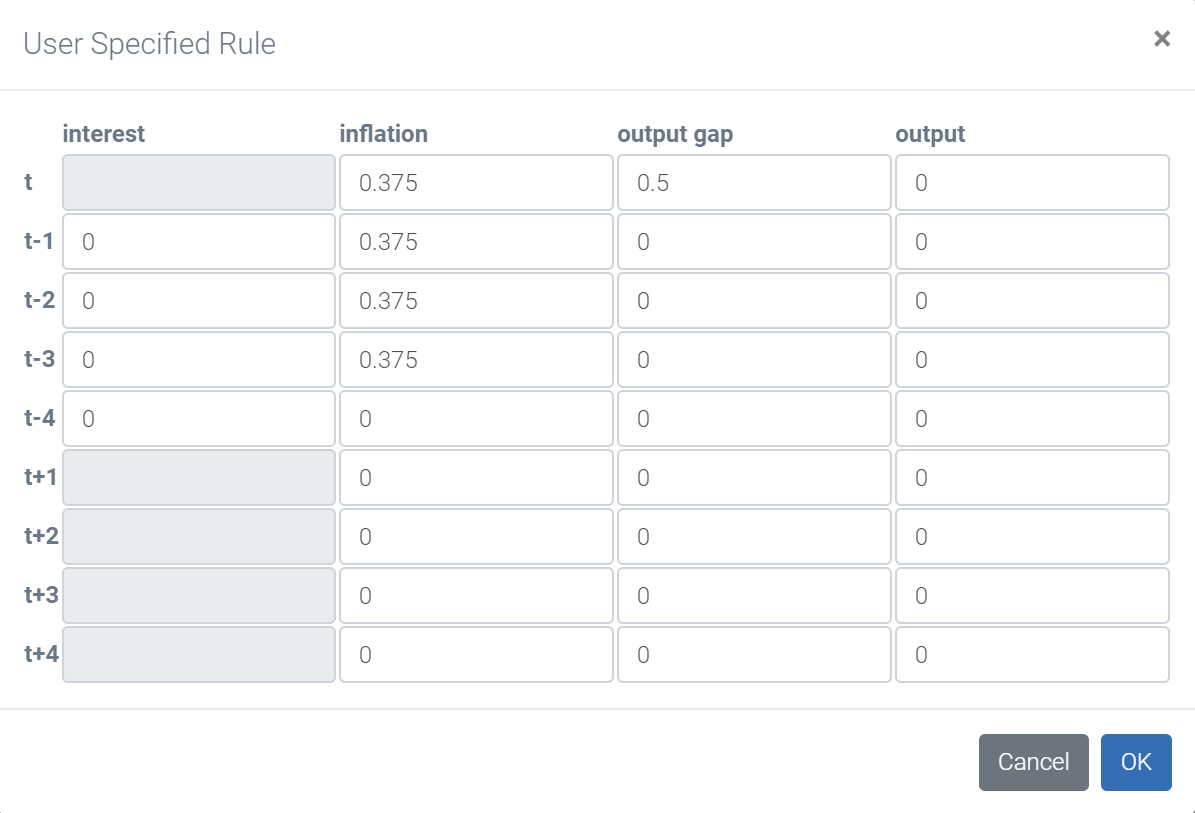
\includegraphics[width=13cm,keepaspectratio]{userrule.png}
        \label{img:userruletaylor}
        \end{figure}

  \item Note that with certain rule parametrization, models cannot be solved due to several reasons. For example, the system of equations may violate the Blanchard-Kahn conditions so a model does not yield a unique stationary rational expectations equilibrium. There is no clear guideline for conditions for determinacy, but \cite{LevinWielandWilliams2003} suggest several crucial characteristics of rules that deliver a unique equilibrium: a relatively short inflation forecast horizon, a moderate degree of responsiveness to the inflation forecast, an explicit response to the current output gap, and a substantial degree of policy inertia.
\end{itemize}


There are three ways to add a new rule to the Modelbase: 1) add a rule to a list of common monetary policy rules, 2) include the model-specific rule calibrated or estimated by the original model authors and 3) specify a rule using the Modelbase user-specified rule option. Below we discuss each case in detail. Keep in mind that policy rules in the Modelbase have to be reformulated in terms of common Modelbase variables such as the annualized quarterly interest rate, the annualized quarter-to-quarter rate of inflation, the quarterly output and the quarterly output gap. This is explained in detail in \cite{WCMSW2012} and in the separate document, called 'MMB\_MPrule\_description.pdf'. Also, one can see how it practically works by looking at common monetary policy rules already implemented in the \emph{MMB\_OPTIONS/MMB\_settings.m} file.
\newline


\noindent {\it 1) Add a common monetary policy rule}\\
\textbf{TO BE COMPLETED}
\begin{itemize}
  \item The first task is to choose a suitable name for the new policy rule and to include it into an array for a list of rule names, \emph{rulenames}. One also has to add its acronyms in character arrays, \emph{rulenamesshort} and \emph{rulenamesshort1} \footnote{ As \emph{rulenamesshort1} are used for displaying simulation outcomes in Matlab console, any blank is not allowed in the rule name.}. Please make sure that the new rule name is of the same size of character array as the already existing one. Next, one assigns color to the rule with the array \textit{myrulecolor}.
	\item Then, one adds the specification of the new-rule coefficients right after the last common rule's specification.
  \item The remaining work is to add the new rule to the frontend of the MMB 3.0 \\\textbf{TO BE COMPLETED}.
\end{itemize}


\noindent {\it 2) Add the model-specific monetary policy rule}

\begin{itemize}
  \item When adding a new model, it is possible to include its policy rule as long as the rule can be rewritten in terms of Modelbase common variables. If this is the case, the user should add the model identification number to the variable vector \emph{model\_with\_rule} in the  file \emph{MMB\_settings.m} such that a model-specific rule is activated when its corresponding model is chosen in \textbf{Option 2}. Otherwise, the user should add the model number to the variable vector \emph{model\_without\_rule}. For example, if the policy rule is set for the interest rate to react to exchange rate or credit growth, the user cannot include the original rule in the Modelbase.
  \item Finally, the user has to insert the specification of the model-specific rule into the part of \emph{switch} statement in the file \emph{MMB\_OPTIONS/MSR\_COEFFFS.m} using the model's identification number as the case expression.
\end{itemize}

\noindent {\it 3) User-specified monetary rule}

\begin{itemize}
  \item When \textit{User-specified rule} is chosen, a menu with a general form of a monetary policy rule appears in terms of common variables. Then, one can specify desired coefficient values of each variable in columns and to the corresponding lag/lead in rows.
      For example, to implement the Taylor (1993) rule using the option for user-specified monetary policy rule, one should set the coefficients as following: $ \rho_{\pi,0} = \rho_{\pi,-1} = \rho_{\pi,-2} = \rho_{\pi,-3} = 0.375, \rho_{q,0} = 0.5 $ and the rest of coefficients to zero. Figure \ref{img:userruletaylor} illustrates how to use the option for a user-specified rule with the example of Taylor (1993) rule. \\

        \begin{figure}[H]
        \centering
        \caption{\textsc{Taylor (1993) rule using the option of user-specified rule }}
        \vspace{0.2cm}
        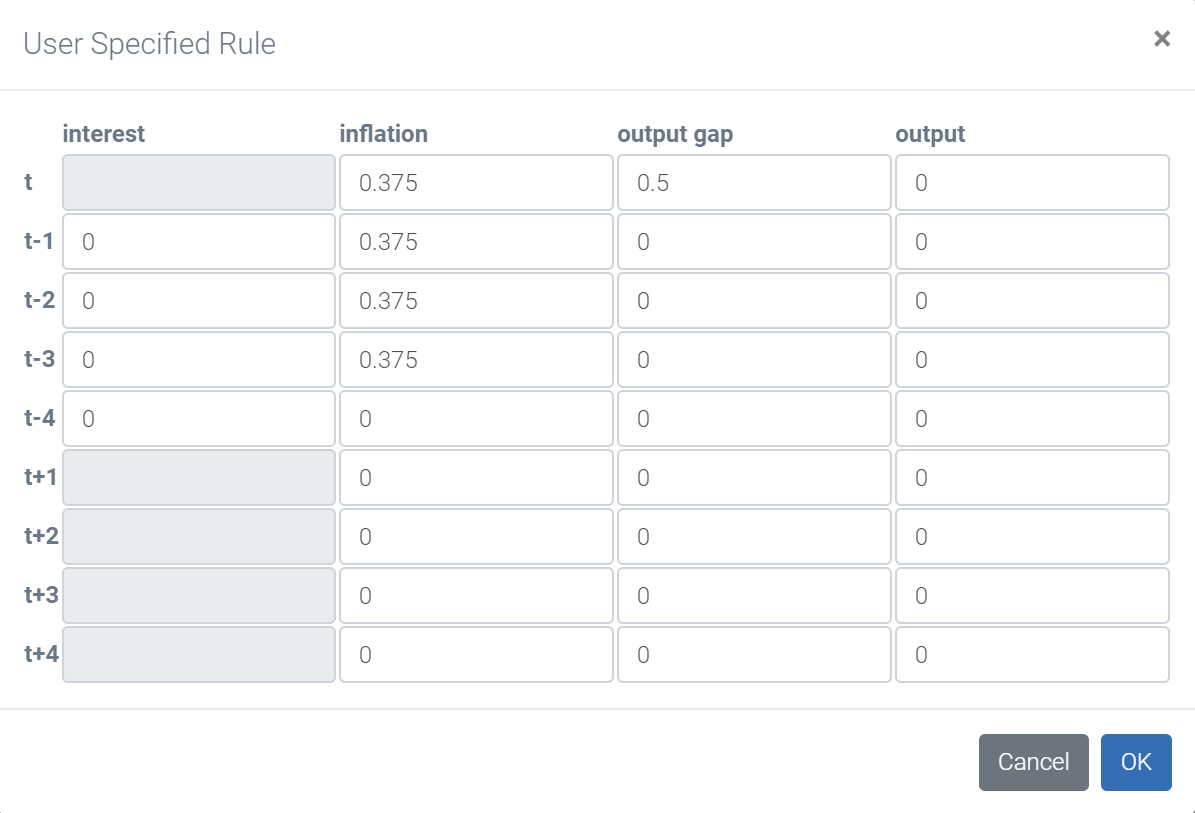
\includegraphics[width=13cm,keepaspectratio]{userrule.png}
        \label{img:userruletaylor}
        \end{figure}

  \item Note that with certain rule parametrization, models cannot be solved due to several reasons. For example, the system of equations may violate the Blanchard-Kahn conditions so a model does not yield a unique stationary rational expectations equilibrium. There is no clear guideline for conditions for determinacy, but \cite{LevinWielandWilliams2003} suggest several crucial characteristics of rules that deliver a unique equilibrium: a relatively short inflation forecast horizon, a moderate degree of responsiveness to the inflation forecast, an explicit response to the current output gap, and a substantial degree of policy inertia.
\end{itemize}

